% Research component, 2026-10-10. Parent may adapt labels and bibliography.
% Baseline: 28357e8ca63dd78327db91d9be239d75e4462879.
\section{The sharp signed-moment threshold for subunit orders}
\label{subunit:sec:main}

The earlier angular-zero continuation \cite{AngularBaseline} extends the signed Mellin kernel
from integer outer order to real $a\geq1$. The restriction $a\geq1$ is
not the actual boundary of this method. The correct boundary is
$a+b=1$ when $0<b<1$. At that boundary a density becomes a measure with
a positive atom at one. The atom must be retained: substituting zero
for a vanishing reciprocal Gamma factor would lose its entire mass.

Write
\[
 A_n(a,b)=\frac{H_{n-1}^{(b)}}{n^a},\qquad
 F_{a,b}(z)=\sum_{n\geq1}A_n(a,b)z^n\quad(|z|<1).
\]
We permit $a=0$ to state the sharp endpoint. Throughout $b>0$.

\begin{theorem}[Exact finite-measure domain]
\label{subunit:thm:domain}
For $a\geq0$ and $b>0$, a finite real signed measure $\nu_{a,b}$ on
$[0,1]$ satisfying
\begin{equation}\label{subunit:eq:moments}
 \int_{[0,1]}u^{n-1}\,d\nu_{a,b}(u)=A_n(a,b)
 \qquad(n\geq1)
\end{equation}
exists if and only if
\begin{equation}\label{subunit:eq:domain}
 (a>0\ \hbox{and}\ a+b\geq1)
 \quad\hbox{or}\quad(a=0\ \hbox{and}\ b>1).
\end{equation}
It is unique and has total mass zero. More precisely:
\begin{enumerate}
\item If $a>0$ and $a+b>1$, it has an integrable density
      $\kappa_{a,b}(u)$ with exactly one strict sign change, from
      negative to positive as $u$ increases, at a point $r_{a,b}\in(0,1)$.
\item If $0<b<1$ and $a=1-b$, then
      $\nu_{a,b}=(1-b)^{-1}\delta_1+\kappa_{a,b}(u)\,du$,
      where $\kappa_{a,b}(u)<0$ throughout $(0,1)$.
\item If $a=0$ and $b>1$, then
      $\nu_{0,b}=\zeta(b)\delta_1+\kappa_{0,b}(u)\,du$,
      where $\kappa_{0,b}(u)<0$ throughout $(0,1)$.
\end{enumerate}
In the two atomic cases all positive mass is at one and all negative
mass is in $(0,1)$. Outside \eqref{subunit:eq:domain}, not even a
finite signed measure with arbitrarily many sign changes can satisfy
\eqref{subunit:eq:moments}.
\end{theorem}

\begin{figure}[tbp]
\centering
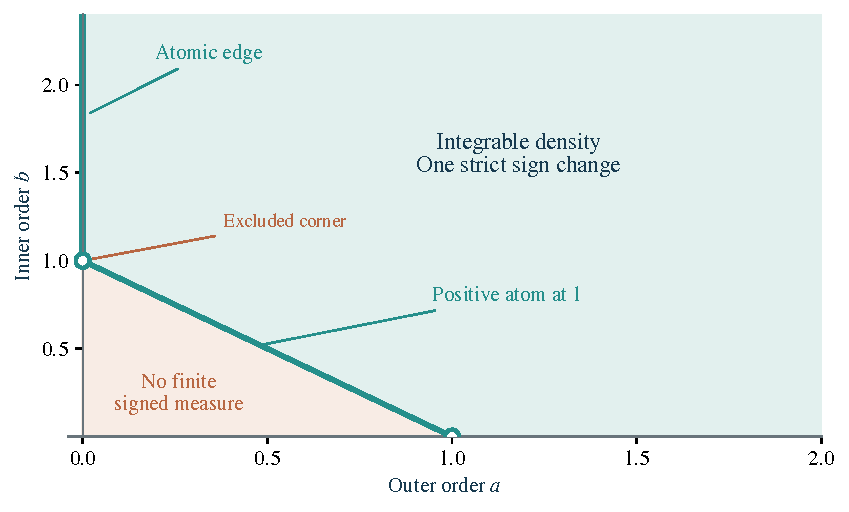
\includegraphics[width=0.8\linewidth]{figures/signed_measure_domain.pdf}
\caption{The exact finite signed-measure domain for $a\ge0,b>0$.
The teal edges carry a positive atom at one. The point $(0,1)$ is
excluded, and the horizontal axis $b=0$ is outside the stated domain.
The absence of a finite measure below the diagonal does not assert
the presence of a complex zero.}
\label{fig:measure-domain}
\end{figure}

\subsection{A regularized positive kernel}

Set
\begin{equation}\label{subunit:eq:q}
 q(t)=\frac1{1-e^{-t}}-\frac1t,\qquad t>0.
\end{equation}
The elementary identities
\[
 q(t)=\frac12+\frac12\coth(t/2)-\frac1t,
 \qquad
 q'(t)=\frac1{t^2}-\frac1{4\sinh^2(t/2)}>0
\]
give $1/2<q(t)<1$, because $\sinh(t/2)>t/2$ and the endpoint
limits are $1/2$ and $1$. In particular $q$ is positive, bounded and
strictly increasing. Also $q(t)=1/2+O(t)$ as $t\downarrow0$.

The classical Hurwitz integral and one elementary subtraction give
\begin{equation}\label{subunit:eq:hurwitz}
 \zeta(b,x)=\frac{x^{1-b}}{b-1}
 +\frac1{\Gamma(b)}\int_0^\infty
              e^{-xt}t^{b-1}q(t)\,dt,
 \qquad x>0,\ b>0,\ b\ne1.
\end{equation}
For $b>1$ this is obtained by splitting $1/(1-e^{-t})=1/t+q(t)$
in the usual Gamma integral. The integral involving $q$ is holomorphic
for $\Re b>0$, so the identity theorem extends the same formula to
$0<b<1$. This is analytic continuation of an absolutely convergent
regularized integral, not subtraction of two divergent real integrals.
The standard starting integral and recurrence are DLMF
25.11.25 and 25.11.4 \cite{DLMFhurwitz}. For $b=1$ the corresponding formula is
\begin{equation}\label{subunit:eq:digamma}
 \psi(x)=\log x-\int_0^\infty e^{-xt}q(t)\,dt,
\end{equation}
which is DLMF 5.9.13 \cite{DLMFdigamma} and also follows by taking the finite part of
\eqref{subunit:eq:hurwitz} at $b=1$.

For $0<b<1$, we shall use $\zeta(b)<0$. Indeed the alternating
Dirichlet series $\eta(b)$ is positive, while
$\eta(b)=(1-2^{1-b})\zeta(b)$ and $1-2^{1-b}<0$.

\subsection{Explicit densities and their Laplace transforms}

Put $T=-\log u$ and $K_{a,b}(T)=\kappa_{a,b}(e^{-T})$. For
$a>0$, $a+b>1$ and $b\ne1$, define
\begin{align}\label{subunit:eq:generalK}
 K_{a,b}(T)={}&\frac{\zeta(b)T^{a-1}}{\Gamma(a)}
 -\frac{T^{a+b-2}}{(b-1)\Gamma(a+b-1)}\notag\\
 &-\frac1{\Gamma(a)\Gamma(b)}
    \int_0^T(T-t)^{a-1}t^{b-1}q(t)\,dt.
\end{align}
When $b>1$, an equivalent form is
\begin{equation}\label{subunit:eq:largeB}
 K_{a,b}(T)=\frac{\zeta(b)T^{a-1}}{\Gamma(a)}
 -\frac1{\Gamma(a)\Gamma(b)}
   \int_0^T\frac{(T-t)^{a-1}t^{b-1}}{1-e^{-t}}\,dt.
\end{equation}
At $b=1$, define
\begin{align}\label{subunit:eq:bOne}
 K_{a,1}(T)={}&\frac{T^{a-1}}{\Gamma(a)}
       \bigl(\gamma+\psi(a)-\log T\bigr)\notag\\
 &-\frac1{\Gamma(a)}\int_0^T(T-t)^{a-1}q(t)\,dt.
\end{align}
The Gamma factors and the term $\gamma+\psi(a)$ in this last formula
are essential; in particular it reduces at $a=1$ to
$K_{1,1}(T)=-\log(e^T-1)$, agreeing with the original signed kernel.

These functions are integrable against $e^{-T}\,dT$. At zero,
\eqref{subunit:eq:generalK} has only the integrable powers
$T^{a-1}$, $T^{a+b-2}$ and $O(T^{a+b-1})$; the logarithmic factor
in \eqref{subunit:eq:bOne} is likewise integrable for $a>0$.
At infinity all terms have at most polynomial times logarithmic growth.
For $b>1$, the integrability of the convolution in
\eqref{subunit:eq:largeB} at its lower endpoint uses $b>1$ explicitly.

By the Gamma integral and the convolution rule, the Laplace transform
of \eqref{subunit:eq:generalK} is
\begin{align*}
 \int_0^\infty e^{-nT}K_{a,b}(T)\,dT
  &=n^{-a}\left[\zeta(b)-\frac{n^{1-b}}{b-1}
     -\frac1{\Gamma(b)}\int_0^\infty
                         e^{-nt}t^{b-1}q(t)\,dt\right]\\
  &=n^{-a}\bigl(\zeta(b)-\zeta(b,n)\bigr)
   =\frac{H_{n-1}^{(b)}}{n^a}.
\end{align*}
Each convolution interchange is justified absolutely; $q$ is bounded
and the remaining factors have Gamma integrals. Formula
\eqref{subunit:eq:bOne} has Laplace transform
\[
 n^{-a}\left(\gamma+\log n-\int_0^\infty e^{-nt}q(t)\,dt\right)
 =n^{-a}(\gamma+\psi(n))=\frac{H_{n-1}}{n^a}.
\]
Here the Laplace transform of $T^{a-1}\log T$ is obtained by
differentiating the Gamma integral, justified by absolute integrability.
The substitution $u=e^{-T}$ changes $u^{n-1}\,du$ to
$e^{-nT}\,dT$, proving the desired moment normalization. In particular
$n=1$ gives total mass zero.

\subsection{The one-sign-change proof}

For $b>1$, divide \eqref{subunit:eq:largeB} by $T^{a-1}$ and
rescale $t=Tv$:
\[
 T^{1-a}K_{a,b}(T)=\frac{\zeta(b)}{\Gamma(a)}
 -\frac1{\Gamma(a)\Gamma(b)}
  \int_0^1(1-v)^{a-1}v^{b-1}\frac{T^b}{1-e^{-Tv}}\,dv.
\]
For fixed $v>0$, the logarithmic derivative of
$T^b/(1-e^{-Tv})$ is
\[
 \frac bT-\frac{v}{e^{Tv}-1}>\frac{b-1}{T}>0.
\]
Thus the rescaled density is strictly decreasing. Its limit at zero is
$\zeta(b)/\Gamma(a)>0$, and its limit at infinity is $-\infty$.
This proves one strict positive--negative crossing in the $T$ coordinate.

For $b=1$, the rescaled expression is
\[
 \Gamma(a)T^{1-a}K_{a,1}(T)
 =\gamma+\psi(a)-\log T
  -T\int_0^1(1-v)^{a-1}q(Tv)\,dv.
\]
It is strictly decreasing from $+\infty$ to $-\infty$, since $q$ is
positive and increasing. For $0<b<1$, instead divide by
$T^{a+b-2}$ to obtain
\begin{align}\label{subunit:eq:rescaledLowB}
 T^{2-a-b}K_{a,b}(T)={}&
 \frac1{(1-b)\Gamma(a+b-1)}
 +\frac{\zeta(b)}{\Gamma(a)}T^{1-b}\notag\\
 &-\frac{T}{\Gamma(a)\Gamma(b)}
   \int_0^1(1-v)^{a-1}v^{b-1}q(Tv)\,dv.
\end{align}
Now the first term is positive, the second is strictly decreasing
because $\zeta(b)<0$, and the final term is strictly decreasing because
$q$ is positive and increasing. The endpoint limits are a positive
constant and $-\infty$. Thus there is again exactly one strict crossing.
The derivatives of these rescaled expressions are strictly negative;
differentiation is dominated by the same integrable beta weights.
At a zero of $K$, multiplication by the positive rescaling factor does
not affect the sign of its derivative. Reversing $T=-\log u$ gives
the asserted negative--positive sign change and a strictly positive
$u$ derivative at its unique crossing.

\subsection{The critical atom and the exact boundary}

Let $0<b<1$ and $a=1-b$. Replace the middle term of
\eqref{subunit:eq:generalK} by an atom of mass $(1-b)^{-1}$ at $u=1$,
and retain the density
\begin{equation}\label{subunit:eq:criticaldensity}
 K_{1-b,b}(T)=\frac{\zeta(b)T^{-b}}{\Gamma(1-b)}
 -\frac1{\Gamma(1-b)\Gamma(b)}
   \int_0^T(T-t)^{-b}t^{b-1}q(t)\,dt.
\end{equation}
Both terms are strictly negative and integrable against $e^{-T}\,dT$.
Its moments plus the atom are
\[
 \frac1{1-b}+n^{b-1}\left[\zeta(b)
   -\frac1{\Gamma(b)}\int_0^\infty e^{-nt}t^{b-1}q(t)\,dt\right]
 =\frac{H_{n-1}^{(b)}}{n^{1-b}},
\]
by \eqref{subunit:eq:hurwitz}. Thus the measure has total mass zero,
and its negative mass is exactly $(1-b)^{-1}$.

For $a=0$, $b>1$, the formula is especially simple:
\begin{equation}\label{subunit:eq:aZero}
 \nu_{0,b}=\zeta(b)\delta_1+K_{0,b}(-\log u)\,du,
 \qquad K_{0,b}(T)=-\frac{T^{b-1}}{\Gamma(b)(1-e^{-T})}.
\end{equation}
The ordinary Hurwitz integral gives its moments immediately. Its
negative mass is exactly $\zeta(b)$.

Every finite signed measure has bounded moments, since
$|\int u^{n-1}\,d\nu|\leq\|\nu\|_{\mathrm{TV}}$.
If $0<b<1$, elementary integral comparison gives
$H_{n-1}^{(b)}\sim n^{1-b}/(1-b)$, so the moments diverge to
infinity when $a+b<1$. If $a=0,b=1$, they diverge logarithmically.
These are exactly the excluded cases for $a\geq0,b>0$.
Finally, two finite signed measures with the same moments integrate
every polynomial equally; polynomial density in $C([0,1])$ makes the
measures identical. This proves Theorem~\ref{subunit:thm:domain}.

\section{Consequences for complex zeros and angular zeros}

\begin{theorem}[Nonvanishing throughout the finite-measure domain]
\label{subunit:thm:zerofree}
For all parameters in \eqref{subunit:eq:domain}, $F_{a,b}$ has an
analytic continuation to $\mathbb C\setminus[1,\infty)$ and has no
zero there except for its double zero at the origin. Every upper
open semicircle $z=\rho e^{i\theta}$, $0<\rho\leq1$, $0<\theta<\pi$,
has exactly one
simple zero of $\operatorname{Im}F_{a,b}(z)$, and it satisfies
\[
 \arccos\rho<\theta_{a,b}(\rho)<\frac\pi2.
\]
The imaginary part is positive below this angle and negative above
it; its angular derivative at the zero is strictly negative.
In the atomic cases, unit-circle values mean analytic continuation
or Abel boundary values: the original Fourier summands do not tend
to zero, so ordinary Fourier convergence is not asserted.
\end{theorem}

\begin{proof}
The signed transform
\[
 F_{a,b}(z)=z\int_{[0,1]}\frac{d\nu_{a,b}(u)}{1-zu}
\]
follows by geometric expansion in the disk and extends analytically
to the slit plane by uniform domination on compact sets. Let $r$ be
the crossing from Theorem~\ref{subunit:thm:domain}, or let $r=1$ in
the atomic cases. Zero mass gives
\begin{equation}\label{subunit:eq:factor}
 F_{a,b}(z)=\frac{z^2}{1-rz}P_{a,b}(z),\qquad
 P_{a,b}(z)=\int_{[0,1]}\frac{u-r}{1-zu}\,d\nu_{a,b}(u).
\end{equation}
The measure $(u-r)\,d\nu_{a,b}(u)$ is positive and nonzero, including
when $r=1$: its atom disappears but its density is strictly positive
on $(0,1)$. Consequently $\operatorname{Im}P_{a,b}(z)$ has the
strict sign of $\operatorname{Im}z$, while $P_{a,b}(x)>0$ for
$x<1$. Apart from the explicit $z^2$, the factor $(1-rz)^{-1}$ in
\eqref{subunit:eq:factor} is analytic and nonzero on the slit plane. Since $P_{a,b}(0)=A_2=2^{-a}$,
the zero at zero has multiplicity exactly two.

For angular zeros put
\[
 J_\rho(c)=\int_{[0,1]}\frac{d\nu(u)}{1-2\rho cu+\rho^2u^2},
 \qquad
 \operatorname{Im}F(\rho e^{i\theta})
       =\rho\sin\theta\,J_\rho(\cos\theta).
\]
The zero-mass one-crossing sign test holds for our atomic measures as
well: subtract the value of the test function at $r$, and use the
ordered supports of the two signs. It gives $J_\rho(0)<0$.
When $\rho<1$, the kernel at $c=\rho$ is strictly increasing in $u$,
so $J_\rho(\rho)>0$. When $\rho=1$ and the crossing is interior,
separate the two signs before expanding $(1-u)^{-2}$ to obtain
\[
 \lim_{c\uparrow1}J_1(c)
 =\int_{[0,1]}\frac{d\nu(u)}{(1-u)^2}
 =\sum_{n\geq1}n A_n>0,
\]
allowing $+\infty$. The negative part is supported away from one, so
this is the same justified monotone-limit argument as in the original
signed-kernel theorem. In the atomic cases the limiting signed
integral at $c=1$ need not be defined, and we do not use that display.
Instead the limit is $+\infty$ directly: the atom contributes
$M/[2(1-c)]$, and the negative density contributes
$o((1-c)^{-1})$. For the latter assertion, multiply its integral by
$1-c$ and use dominated convergence: the multiplier
$(1-c)/(1-2cu+u^2)$ is bounded by $1$ for $0\leq c<1$ and tends to zero for
every $u<1$. The negative density is integrable and has no atom at one.

For $c'>c$, the quotient of the two kernels has derivative
\[
 \frac{d}{du}\frac{1-2\rho cu+\rho^2u^2}
                         {1-2\rho c'u+\rho^2u^2}
 =\frac{2\rho(c'-c)(1-\rho^2u^2)}
       {(1-2\rho c'u+\rho^2u^2)^2}>0\quad(0<u<1).
\]
At any zero, apply the sign test to the signed measure obtained by
weighting $\nu$ with the positive kernel. It follows that $J_\rho$
is positive at every larger $c$ and negative at every smaller $c$;
this proves uniqueness and the signs. Finally its derivative at its
zero is positive, because the additional factor
$2\rho u/(1-2\rho cu+\rho^2u^2)$ is strictly increasing in $u$.
The angular derivative is therefore
$-\rho\sin^2\theta\,J_\rho'(\cos\theta)<0$.
\end{proof}

The theorem is sharp as a statement about finite signed moment
representations. It does not assert that nonvanishing fails below
$a+b=1$: the absence of this particular representation is not a
complex-zero counterexample. In fact the entire axis $a=0,b>0$ is zero-free away from the origin.
The geometric sum gives
\[
 F_{0,b}(z)=\frac{z\Li_b(z)}{1-z}
 =\frac{z^2}{1-z}\frac1{\Gamma(b)}
       \int_0^1\frac{(-\log u)^{b-1}}{1-zu}\,du.
\]
The last integral is a nonzero positive-measure transform on the slit
plane, by exactly the imaginary-part and real-axis argument used above.
Thus finite signed-moment representability and complex nonvanishing
have different parameter boundaries, already on this explicit axis.

\section{Formation of the endpoint atom}

\begin{theorem}[Boundary-layer scale and weak convergence]
\label{subunit:thm:boundarylayer}
Fix $0<b<1$, let $a=1-b+\varepsilon$ with $\varepsilon>0$, and
let $T_\varepsilon=-\log r_{a,b}$. Define
\[
 \tau_\varepsilon=
 \left(\frac{\Gamma(1-b+\varepsilon)}
 {(1-b)(-\zeta(b))\Gamma(\varepsilon)}\right)^{1/(1-b)}.
\]
Then, as $\varepsilon\downarrow0$,
\begin{equation}\label{subunit:eq:layerexact}
 T_\varepsilon=\tau_\varepsilon
 \left(1+O_b\left(\frac{\tau_\varepsilon}{\varepsilon}\right)\right),
 \qquad 0<T_\varepsilon<\tau_\varepsilon,
\end{equation}
and in particular
\begin{equation}\label{subunit:eq:layerleading}
 1-r_{1-b+\varepsilon,b}\sim
 \left(\frac{\Gamma(1-b)}{(1-b)(-\zeta(b))}
       \varepsilon\right)^{1/(1-b)}.
\end{equation}
The measures converge weakly to the critical measure in
Theorem~\ref{subunit:thm:domain}, and their positive masses converge
to $(1-b)^{-1}$ while their positive supports shrink to $u=1$.
\end{theorem}

\begin{proof}
In \eqref{subunit:eq:rescaledLowB}, put
$A_\varepsilon=((1-b)\Gamma(\varepsilon))^{-1}$ and
$B_\varepsilon=(-\zeta(b))/\Gamma(1-b+\varepsilon)$.
The zero equation is
\[
 A_\varepsilon-B_\varepsilon T^{1-b}-T C_\varepsilon(T)=0,
 \quad
 C_\varepsilon(T)=\frac1{\Gamma(a)\Gamma(b)}
 \int_0^1(1-v)^{a-1}v^{b-1}q(Tv)\,dv.
\]
Since $1/2<q<1$ and $a+b=1+\varepsilon$,
\[
 \frac1{2\Gamma(1+\varepsilon)}
 <C_\varepsilon(T)<\frac1{\Gamma(1+\varepsilon)}.
\]
By definition $B_\varepsilon\tau_\varepsilon^{1-b}
=A_\varepsilon$, so the equation at $T=\tau_\varepsilon$ has
strictly negative left side and $T_\varepsilon<\tau_\varepsilon$.
Furthermore
\[
 0\leq1-(T_\varepsilon/\tau_\varepsilon)^{1-b}
 =\frac{T_\varepsilon C_\varepsilon(T_\varepsilon)}
       {A_\varepsilon}
 \leq\frac{(1-b)\tau_\varepsilon}{\varepsilon}.
\]
The final equality in the upper bound uses
$\Gamma(1+\varepsilon)=\varepsilon\Gamma(\varepsilon)$.
Now $\tau_\varepsilon=O_b(\varepsilon^{1/(1-b)})$, hence
$\tau_\varepsilon/\varepsilon\to0$. The last inequality proves
\eqref{subunit:eq:layerexact}. Expanding the Gamma ratio and using
$1-e^{-T}\sim T$ proves \eqref{subunit:eq:layerleading}.

For weak convergence, the positive term in
\eqref{subunit:eq:generalK}, regarded as a measure in the $T$
coordinate, is
\[
 \frac1{1-b}\frac{e^{-T}T^{\varepsilon-1}}
 {\Gamma(\varepsilon)}\,dT.
\]
It is $(1-b)^{-1}$ times a Gamma$(\varepsilon,1)$ law. Its mean
is $\varepsilon$, so it converges weakly to mass $(1-b)^{-1}$
at $T=0$, equivalently at $u=1$. The two negative components in
\eqref{subunit:eq:generalK} converge in $L^1(e^{-T}\,dT)$ to
those in \eqref{subunit:eq:criticaldensity}. For the power term,
dominated convergence holds with an exponent bounded above $-1$.
For the convolution, either use the rescaled beta integral and the
same domination, or use $L^1$ continuity of the Gamma densities and
the integrable convolution factor $e^{-t}t^{b-1}q(t)$.

The unique positive support is $0<T<T_\varepsilon$, which shrinks
to zero. The Gamma$(\varepsilon,1)$ mass in this interval tends to
one: since $T_\varepsilon$ is a fixed power of $\varepsilon$ to
leading order,
\[
 \frac1{\Gamma(\varepsilon)}\int_0^{T_\varepsilon}
 e^{-T}T^{\varepsilon-1}\,dT
 =\frac{T_\varepsilon^\varepsilon}{\Gamma(1+\varepsilon)}(1+o(1))
 \longrightarrow1.
\]
The negative components have vanishing mass on the shrinking interval
by their $L^1$ convergence to an integrable limit. Thus the actual
positive mass of the signed density tends to $(1-b)^{-1}$, completing
the proof.
\end{proof}

\subsection{The other edge and the logarithmic corner}

The second atomic edge has a complementary power law. The corner $b=1$
has an exponential scale and no finite limiting measure.

\begin{proposition}[Two further endpoint scales]
\label{subunit:prop:otheredges}
For fixed $b>1$, as $a\downarrow0$,
\begin{equation}\label{subunit:eq:otheredge}
 1-r_{a,b}\sim\bigl(\Gamma(b)\zeta(b)a\bigr)^{1/(b-1)}.
\end{equation}
The measures converge weakly to $\nu_{0,b}$, and their positive masses
converge to $\zeta(b)$. For $b=1$, set
$\sigma_a=\exp(\gamma+\psi(a))$. Then
\begin{equation}\label{subunit:eq:logcorner}
 -\log r_{a,1}=\sigma_a\bigl(1+O(\sigma_a/a)\bigr),
 \qquad 0<-\log r_{a,1}<\sigma_a,
\end{equation}
where
\[
 \sigma_a=\exp\bigl(-1/a+\zeta(2)a-\zeta(3)a^2+O(a^3)\bigr).
\]
If $M_{a,1}$ denotes either signed mass of $\nu_{a,1}$, then
\begin{equation}\label{subunit:eq:divergingmass}
 M_{a,1}\sim\frac1{e a}.
\end{equation}
Thus the finite signed measures have unbounded total variation at this
corner, consistently with the impossibility of a finite measure at
$a=0,b=1$.
\end{proposition}

\begin{proof}
For $b>1$, the equation obtained from
\eqref{subunit:eq:generalK} after division by $T^{a-1}$ is
\[
 0=\frac{\zeta(b)}{\Gamma(a)}
 -\frac{T^{b-1}}{(b-1)\Gamma(a+b-1)}
 -\frac{T^b}{\Gamma(a)\Gamma(b)}
       \int_0^1(1-v)^{a-1}v^{b-1}q(Tv)\,dv.
\]
The last integral, after its Gamma normalization, lies between
$1/(2\Gamma(a+b))$ and $1/\Gamma(a+b)$. The ratio of this
last term to the preceding negative term is therefore $O_b(T)$,
uniformly for small positive $a$. The balancing point of the first
two terms is
\[
 \left(\frac{(b-1)\Gamma(a+b-1)\zeta(b)}{\Gamma(a)}\right)^{1/(b-1)}
 \sim\bigl(\Gamma(b)\zeta(b)a\bigr)^{1/(b-1)}.
\]
The strict monotonicity of the rescaled density, or the same two-sided
comparison used in Theorem~\ref{subunit:thm:boundarylayer}, makes the
actual zero asymptotic to this point. The positive term is $\zeta(b)$
times a Gamma$(a,1)$ law in the $T$ coordinate. The negative term in
\eqref{subunit:eq:largeB}, after multiplication by $e^{-T}$, is the
convolution of that Gamma probability density with
$e^{-t}t^{b-1}/(\Gamma(b)(1-e^{-t}))$, an integrable function of mass
$\zeta(b)$. As $a\downarrow0$, this convolution converges in $L^1$
to the latter function; Gamma$(a,1)$ is an approximate identity since
its mean tends to zero. This proves weak convergence. As before,
the Gamma mass below the crossing tends to one, since $a\log T\to0$,
and the limiting negative density is integrable. Hence the positive
mass tends to $\zeta(b)$.

For $b=1$, put
$J_a(T)=\int_0^1(1-v)^{a-1}q(Tv)\,dv$, so that
$1/(2a)<J_a(T)<1/a$. At the crossing $T_a$, formula
\eqref{subunit:eq:bOne} says
\[
 \log(\sigma_a/T_a)=T_aJ_a(T_a),\qquad
 0<\log(\sigma_a/T_a)<\sigma_a/a.
\]
This gives \eqref{subunit:eq:logcorner}. The digamma expansion
$\psi(a)=-1/a-\gamma+\zeta(2)a-\zeta(3)a^2+O(a^3)$ gives
the stated scale.

Finally the positive mass is the integral of
$e^{-T}T^{a-1}[\log(\sigma_a/T)-T J_a(T)]/\Gamma(a)$
over $0<T<T_a$. Omitting the factor $e^{-T}$, the $TJ_a$ term,
and the vanishing interval between $T_a$ and $\sigma_a$ changes
the result by a relative $o(1)$. To see this explicitly, the first
omission has relative error at most $\sigma_a$; the $TJ_a$ integral
is at most $\sigma_a^{a+1}/(a(a+1)\Gamma(a))$, whereas the main
integral is $\sigma_a^a/(a^2\Gamma(a))$. For the removed interval,
write $T=\sigma_a v$ and use
$1-T_a/\sigma_a=O(\sigma_a/a)$; its relative contribution is
$O(\sigma_a^2)$. Therefore
\[
 M_{a,1}\sim\frac{\sigma_a^a}{a^2\Gamma(a)}
 \sim\frac1{ea},
\]
as asserted.
\end{proof}

\section{Euler certificates in the extended range}

Put $f(k)=A_{2k+1}(a,b)$ and let $D f(k)=f(k)-f(k+1)$.
The same signed-moment proof gives
\[
 D^k f(0)=\int(1-u^2)^k\,d\nu_{a,b}(u)<0\quad(k\geq1),
 \qquad D^0f(0)=0.
\]
This strict sign remains valid in the atomic cases because the atom
is annihilated for $k\geq1$ and the density is negative.
The geometric series is dominated by one, so finite variation and
dominated convergence give, including the atomic cases,
\[
 \sum_{k\geq0}\frac{D^kf(0)}{2^{k+1}}
 =\int\sum_{k\geq0}\frac{(1-u^2)^k}{2^{k+1}}\,d\nu_{a,b}(u)
 =\int\frac{d\nu_{a,b}(u)}{1+u^2}=\Im F_{a,b}(i).
\]
Thus the Euler approximants decrease to $g_{a,b}=\Im F_{a,b}(i)$
even where the original alternating Fourier series does not converge.
Explicitly, the approximant with $N$ terms is
\[
 E_N=\sum_{k=0}^{N-1}\frac{D^kf(0)}{2^{k+1}},\qquad N\ge1.
\]
For $b\ne1$, the explicit decompositions prove
\[
 E_N-C_b2^{-N}\leq g_{a,b}\leq E_N,\qquad
 C_b=\begin{cases}(1-b)^{-1},&0<b<1,\\\zeta(b),&b>1.\end{cases}
\]
Indeed either signed mass is at most $C_b$: use the positive Gamma
component for $b<1$ and the positive $\zeta(b)$ Gamma component for
$b>1$, together with zero mass. Each finite difference has absolute
value at most that signed mass, since its weight lies in $[0,1]$.
For $b=1$, a valid finite mass bound is
\[
 C_{a,1}=\frac{\exp(a(\gamma+\psi(a)))}{a^2\Gamma(a)}.
\]
Indeed the positive part of \eqref{subunit:eq:bOne} is bounded by
$T^{a-1}(\gamma+\psi(a)-\log T)_+/\Gamma(a)$, and its unweighted
$T$ integral is exactly $C_{a,1}$; the factor $e^{-T}$ can only
decrease it. This gives the same enclosure with $C_b$ replaced by
$C_{a,1}$. Summing the geometric Euler tail proves each enclosure.
At noninteger indices its centers are not generally rational. The
earlier sharp constant one applies to its stated range $a\geq1$;
the larger constants above are valid enclosures for the new range,
without an optimality claim for the Euler remainder itself.

% Suggested references:
% DLMF 25.11.25, 25.11.4: https://dlmf.nist.gov/25.11
% DLMF 5.9.13: https://dlmf.nist.gov/5.9
% angular-zero-continuation/article.tex at pinned revision above,
% original signed-kernel chapter at the same revision.
